\section{Data Understanding}
\label{sec:DataUnderstanding}

%In this section, we provide the details of Amazon Data. In particularly, sub-section \ref{sec:amzScale} will describe the scaling of amazon data, section \ref{sec:featureunderstanding} will summarize the useful features of data. 

\subsection{Amazon Data Scale}
\label{sec:amzScale}

% Scale of amazon data
As mentioned above, every changing for a customer's offer in product page is stored by an auction xml file. An auction includes aggregated information about the lowest 20 prices offered for a product (or less, if there are fewer than 20 offers).  \textbf{Fig.\ref{fig:scale}} illustrates the scaling of data in one market. It is provided from several layers as follows:

1. \textbf{Marketplace's scale layer}: The Amazon has many marketplaces for
the United States, Australia, Brazil, Canada, China, France, Germany, India, Italy, Japan, Mexico, Netherlands, Spain, and the United Kingdom. One marketplace is an separated  environment with its own characteristics.  e.g. in India market, there is one seller who wins almost product's competing, while in U.S. market, the auction is normally with two or three competitors.

2. \textbf{Product's scale layer}: From the market place, sellers can sell many products. It could be very different in price, shipping time, conditional note for two different products. The category list of product can be found in the Amazon Web Service.

3. \textbf{Auction's scale layer}: In product's layer, the auction can be recorded when sellers update their product's offers. For example, one seller changes their shipping time from 0 hour to 24 hours, the new auction of that changing with all information of its competitors is parsed as one new XML.

4. \textbf{Offer's scale layer}: One auction contains many offers of sellers in one product. They could be old or new updated offers.


\begin{figure}[!h]
	\begin{center}
		\scalebox{0.5}{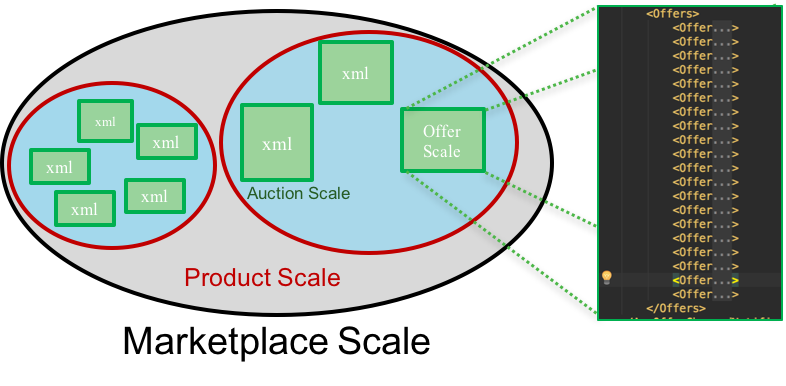
\includegraphics{fig3_scale.png}}
	\end{center}
	\caption{\label{fig:scale}The scales of data in one Marketplace.}
\end{figure}

\subsection{Features Understanding}
\label{sec:featureunderstanding}

%% table of features


%% New feature
To facilitate the analysis, we model the Buy Box as a prediction problem. Specifically, for a product offered by $n$ sellers, each of which is characterized by a feature vector, our goal is to predict which seller will be chosen to get in the Buy Box. Given the list of XMLs, we create a feature vector for each seller containing the following seven features:

1. xxx

2. xxxx

3. xxxx

4. xxxx

According to Amazon’s documentation, as well as speculation from 3P sellers, other
features are possibly used by the Buy Box algorithm [11, 31]. This includes sales volume, response time to customer inquiries, rate of returns and refunds, and shipping times. Unfortunately, I cannot measure these features, and thus cannot quantify their impact on the Buy Box algorithm. However, as I will show, even without these features I am able to achieve high prediction accuracy, suggesting that my data does capture the most important seller features.

\begin{figure}[!h]
	\begin{center}
		\scalebox{0.27}{\includegraphics{fig7_fi.png}}
	\end{center}
	\caption{\label{fig:fi}An example of the Feature Importance, provided by Random Forest classifier.}
\end{figure}
